\documentclass[english,twoside, openright, hidelinks, 11 pt, class=report,crop=false]{standalone}
\newcommand{\texandasy}{Teksten er skrevet i \LaTeX\ og figurene er lagd ved hjelp av Asymptote.}

\newcommand{\expl}{forklaring}

\newcommand{\note}{Merk}
\newcommand{\notesm}[1]{{\footnotesize \textsl{\note:} #1}}
\newcommand{\ekstitle}{Eksempel }
\newcommand{\sprtitle}{Språkboksen}
\newcommand{\vedlegg}[1]{\section*{Vedlegg \thevedl: #1}  \setcounter{vedleq}{0} \refstepcounter{vedl}}

\newcommand\sv{\vsk \textbf{Svar} \vspace{4 pt}\\}

% exercises
\newcommand{\opgt}{\newpage \phantomsection \addcontentsline{toc}{section}{Oppgåver} \section*{Oppgaver for kapittel \thechapter}\vs \setcounter{section}{1}}

\newcommand{\grubop}[1]{\vspace{15pt} \refstepcounter{grub}\large \textbf{\color{NavyBlue} Gruble \thegrub} \vspace{2 pt} \label{#1} \\}
\newcommand{\grubeksop}[2]{\vspace{15pt} \refstepcounter{grub}\large \textbf{\color{NavyBlue} Gruble \thegrub} (#2) \vspace{2 pt} \label{#1} \\}
\newcommand{\gruboprecc}[1]{\vspace{15pt} \refstepcounter{grub}\large \textbf{\color{NavyBlue} Gruble* \thegrub} \vspace{2 pt} \label{#1} \\}
\newcommand{\grubeksoprecc}[2]{\vspace{15pt} \refstepcounter{grub}\large \textbf{\color{NavyBlue} Gruble* \thegrub} (#2) \vspace{2 pt} \label{#1} \\}
\newcommand{\grubr}[1]{\vspace{3pt}\textbf{Gruble \ref{#1}}}

%references
\newcommand{\reftab}[1]{\hrs{#1}{tabell}}
\newcommand{\rref}[1]{\hrs{#1}{regel}}
\newcommand{\dref}[1]{\hrs{#1}{definisjon}}
\newcommand{\refkap}[1]{\hrs{#1}{kapittel}}
\newcommand{\refsec}[1]{\hrs{#1}{seksjon}}
\newcommand{\refdsec}[1]{\hrs{#1}{delseksjon}}
\newcommand{\refved}[1]{\hrs{#1}{vedlegg}}
\newcommand{\eksref}[1]{\textsl{#1}}
\newcommand\fref[2][]{\hyperref[#2]{\textsl{figur \ref*{#2}#1}}}
\newcommand{\refop}[1]{{\color{blue}Oppgave \ref{#1}}}
\newcommand{\refops}[1]{{\color{blue}oppgave \ref{#1}}}

% Solutions manual
\newcommand{\selos}{Se løsningsforslag.}

\newcommand{\ompref}{Omgjøring av prefikser}

\usepackage[utf8]{inputenc}
\usepackage{lmodern} % load a font with all the characters
\usepackage{geometry}
\geometry{verbose,paperwidth=16 cm, paperheight=24 cm, inner=2.3cm, outer=1.7 cm, bmargin=2cm, tmargin=1.8cm}

\setlength{\parindent}{0bp}
\usepackage{import}
\usepackage[subpreambles=false]{standalone}
\usepackage{amsmath}
\usepackage{amssymb}
\usepackage{esint}
\usepackage{babel}
\usepackage{tabu}
\makeatother
\makeatletter

\usepackage{titlesec}
\usepackage{ragged2e}
\RaggedRight
\raggedbottom
\frenchspacing

\usepackage{graphicx}
\usepackage{float}
\usepackage{subfig}
\usepackage{placeins}
\usepackage{cancel}
\usepackage{framed}
\usepackage{wrapfig}
\usepackage[subfigure]{tocloft}
\usepackage[font=footnotesize,labelfont=sl]{caption} % Figure caption
\usepackage{bm}
\usepackage[dvipsnames, table]{xcolor}
\definecolor{shadecolor}{rgb}{0.105469, 0.613281, 1}
\definecolor{blue}{cmyk}{1, 0, 0, 0}
\definecolor{red}{cmyk}{0, 1, 1, 0}
\definecolor{green}{cmyk}{100,0,100,0}
\colorlet{shadecolor}{Emerald!15} 
\usepackage{icomma}
\makeatother
\usepackage[many]{tcolorbox}
\usepackage{multicol}
\usepackage{stackengine}
\usepackage{listings}
\usepackage{esvect} %For vectors with capital letters

% For tabular
\usepackage{array}
\usepackage{multirow}
\usepackage{longtable} %breakable table

% Ligningsreferanser
\usepackage{mathtools} % for mathclap

\mathtoolsset{showonlyrefs}

% sections without numbering in toc
\newcommand\tsec[1]{\phantomsection \addcontentsline{toc}{section}{#1}
	\section*{#1}}

% index
\usepackage{imakeidx}
\makeindex[title=Indeks]

%Footnote:
\usepackage[bottom, hang, flushmargin]{footmisc}
\usepackage{perpage} 
\MakePerPage{footnote}
\addtolength{\footnotesep}{2mm}
\renewcommand{\thefootnote}{\arabic{footnote}}
\renewcommand\footnoterule{\rule{\linewidth}{0.4pt}}
\renewcommand{\thempfootnote}{\arabic{mpfootnote}}

%colors
\definecolor{c1}{cmyk}{0,0.5,1,0}
\definecolor{c2}{cmyk}{1,0.25,1,0}
\definecolor{n3}{cmyk}{1,0.,1,0}
\definecolor{neg}{cmyk}{1,0.,0.,0}


\newcommand{\nreq}[1]{
\begin{equation}
	#1
\end{equation}
}


% Equation comments
\newcommand{\cm}[1]{\llap{\coln{ #1}}}


\usepackage[inline]{enumitem}
\newcounter{rg}
\numberwithin{rg}{chapter}

\newcommand{\reg}[2][]{\begin{tcolorbox}[boxrule=0.3 mm,arc=0mm,colback=Blue!3] {\refstepcounter{rg}\phantomsection \large \textbf{\therg \;#1} \vspace{5 pt}}\newline #2  \end{tcolorbox} \vs}
\newcommand{\regdef}[2][]{\begin{tcolorbox}[boxrule=0.3 mm,arc=0mm,colback=Blue!3] {\refstepcounter{rg}\phantomsection \large \textbf{\therg \;#1} \vspace{5 pt}}\newline #2  \end{tcolorbox} \vs}
\newcommand{\words}[1]{\begin{tcolorbox}[boxrule=0.3 mm,arc=0mm,colback=Teal!3] #1  \end{tcolorbox} \vs}

\newcommand\alg[1]{\begin{align*} #1 \end{align*}}

\newcommand\eks[2][]{\begin{tcolorbox}[boxrule=0.3 mm,arc=0mm,enhanced jigsaw,breakable,colback=Green!5] {\large \textbf{\ekstitle #1} \vspace{5 pt}\\} #2 \end{tcolorbox}\vs}

\newcommand{\st}[1]{\begin{tcolorbox}[boxrule=0.0 mm,arc=0mm,enhanced jigsaw,breakable,colback=Yellow!7]{ #1} \end{tcolorbox}}
\newcommand{\stf}[1]{\begin{tcolorbox}[boxrule=0.3 mm,arc=0mm,enhanced jigsaw,breakable,colback=Yellow!7]{ #1} \end{tcolorbox}}

\newcommand{\spr}[1]{\begin{tcolorbox}[boxrule=0.3 mm,arc=0mm,enhanced jigsaw,breakable,colback=Yellow!7] {\large \textbf{\sprtitle} \vspace{5 pt}\\} #1 \end{tcolorbox}\vs}

\newcommand{\sym}[1]{\colorbox{NavyBlue!15}{#1}}

\newcommand{\info}[2]{\begin{tcolorbox}[boxrule=0.3 mm,arc=0mm,enhanced jigsaw,breakable,colback=Cyan!6] {\large \textbf{#1} \vspace{5 pt}\\} #2 \end{tcolorbox}
}

\newcommand\algv[1]{\vspace{-11 pt}\begin{align*} #1 \end{align*}}

\newcommand{\regv}{\vspace{5pt}}
\newcommand{\mer}{\textsl{\note}: }
\newcommand{\mers}[1]{{\footnotesize \mer #1}}
\newcommand\vsk{\vspace{11pt}}
\newcommand{\tbs}{\vspace{5pt}}
\newcommand\vs{\vspace{-11pt}}
\newcommand\vsb{\vspace{-16pt}}
\newcommand\vso{\vspace{-5pt}}
\newcommand\br{\\[5 pt]}
\newcommand{\figp}[1]{../fig/#1}
\newcommand\algvv[1]{\vs\vs\begin{align*} #1 \end{align*}}
\newcommand{\y}[1]{$ {#1} $}
\newcommand{\os}{\\[5 pt]}
\newcommand{\prbxl}[2]{
\parbox[l][][l]{#1\linewidth}{#2
	}}
\newcommand{\prbxr}[2]{\parbox[r][][l]{#1\linewidth}{
		\setlength{\abovedisplayskip}{5pt}
		\setlength{\belowdisplayskip}{5pt}	
		\setlength{\abovedisplayshortskip}{0pt}
		\setlength{\belowdisplayshortskip}{0pt} 
		\begin{shaded}
			\footnotesize	#2 \end{shaded}}}
\newcommand{\fgbxr}[2]{
	\parbox[r][][l]{#1\linewidth}{#2
}}		

\renewcommand{\cfttoctitlefont}{\Large\bfseries}
\setlength{\cftaftertoctitleskip}{0 pt}
\setlength{\cftbeforetoctitleskip}{0 pt}

\newcommand{\bs}{\\[3pt]}
\newcommand{\vn}{\\[6pt]}
\newcommand{\fig}[1]{\begin{figure}[H]
		\centering
		\includegraphics[]{\figp{#1}}
\end{figure}}

\newcommand{\localfig}[2]{\begin{figure}[H]
		\centering
		\includegraphics[scale=#2]{#1}
\end{figure}}

\newcommand{\figc}[2]{\begin{figure}
		\centering
		\includegraphics[]{\figp{#1}}
		\caption{#2}
\end{figure}}
\newcommand{\arc}[1]{{
		\setbox9=\hbox{#1}%
		\ooalign{\resizebox{\wd9}{\height}{\texttoptiebar{\phantom{A}}}\cr\textit{#1}}}}

\newcommand{\sectionbreak}{\clearpage} % New page on each section

\newcommand{\nn}[1]{
\begin{equation*}
	#1
\end{equation*}
}

\newcommand{\enh}[1]{\,\text{#1}}

%asin, atan, acos
\DeclareMathOperator{\atan}{atan}
\DeclareMathOperator{\acos}{acos}
\DeclareMathOperator{\asin}{asin}

% Comments % old cm, ggb cm is new
%\newcommand{\cm}[1]{\llap{\color{blue} #1}}

%%%

\newcommand\fork[2]{\begin{tcolorbox}[boxrule=0.3 mm,arc=0mm,enhanced jigsaw,breakable,colback=yellow!7] {\large \textbf{#1 (\expl)} \vspace{5 pt}\\} #2 \end{tcolorbox}\vspace{-5pt} }
 
%colors
\definecolor{projectgreen}{cmyk}{100,0,100,0}

\newcommand{\colr}[1]{{\color{Red} #1}}
\newcommand{\colb}[1]{{\color{Cyan} #1}}
\newcommand{\colo}[1]{{\color{Orange} #1}}
\newcommand{\colc}[1]{{\color{SeaGreen} #1}}
\newcommand{\colg}[1]{{\color{Green} #1}}
\newcommand{\coln}[1]{{\color{NavyBlue} #1}}

% Methods
\newcommand{\metode}[2]{
	\textsl{#1} \\ \vspace{-10pt}
	\rule{#2}{0.75pt}
}

%Opg
\newcommand{\abc}[1]{
	\begin{enumerate}[label=\alph*),leftmargin=18pt]
		#1
	\end{enumerate}
}
\newcommand{\abcs}[2]{
	\begin{enumerate}[label=\alph*),start=#1,leftmargin=18pt]
		#2
	\end{enumerate}
}
\newcommand{\abcn}[1]{
	\begin{enumerate}[label=\arabic*),leftmargin=18pt]
		#1
	\end{enumerate}
}




\newcommand{\abch}[1]{
	\hspace{-2pt}	\begin{enumerate*}[label=\alph*), itemjoin=\hspace{1cm}]
		#1
	\end{enumerate*}
}

\newcommand{\abchs}[2]{
	\hspace{-2pt}	\begin{enumerate*}[label=\alph*), itemjoin=\hspace{1cm}, start=#1]
		#2
	\end{enumerate*}
}

% Exercises


\newcounter{opg}
\numberwithin{opg}{section}

\newcounter{grub}
\numberwithin{opg}{section}
\newcommand{\op}[1]{\vspace{15pt} \refstepcounter{opg}\large \textbf{\color{NavyBlue}\theopg} \vspace{2 pt} \label{#1} \\}
\newcommand{\opd}[1]{\vspace{15pt} \refstepcounter{opg}\large \textbf{\color{NavyBlue}\theopg} 
\includegraphics{../../calculatorimage} \vspace{2 pt} \label{#1} \\}
\newcommand{\eksop}[2]{\vspace{15pt} \refstepcounter{opg}\large \textbf{\color{NavyBlue}\theopg} (#1) \vspace{2 pt} \label{#2} \\}

\newcommand{\nes}{\stepcounter{section}
	\setcounter{opg}{0}}
\newcommand{\opr}[1]{\vspace{3pt}\textbf{\ref{#1}}}
\newcommand{\oeks}[1]{\begin{tcolorbox}[boxrule=0.3 mm,arc=0mm,colback=white]
		\textit{\ekstitle: } #1	  
\end{tcolorbox}}
\newcommand\opgeks[2][]{\begin{tcolorbox}[boxrule=0.1 mm,arc=0mm,enhanced jigsaw,breakable,colback=white] {\footnotesize \textbf{\ekstitle #1} \\} \footnotesize #2 \end{tcolorbox}\vspace{-5pt} }


% tag exercises
\newcommand{\tagop}[1]{ 
{\small \color{Gray} #1} \os
}

% License
\newcommand{\lic}{
This book is part of the \net{https://sindrsh.github.io/openmathbooks/}{OpenMathBooks} project. OpenMathBooks © 2022 by Sindre Sogge Heggen is licensed under CC BY-NC-SA 4.0. To view a copy of this license, visit \net{http://creativecommons.org/licenses/by-nc-sa/4.0/}{http://creativecommons.org/licenses/by-nc-sa/4.0/}}

%referances
\newcommand{\net}[2]{{\color{NavyBlue}\href{#1}{#2}}}
\newcommand{\hrs}[2]{\hyperref[#1]{\color{NavyBlue}#2 \ref*{#1}}}
\newcommand{\refunnbr}[2]{\hyperref[#1]{\color{NavyBlue}#2}}


\newcommand{\openmath}{\net{https://sindrsh.github.io/openmathbooks/}{OpenMathBooks}}
\newcommand{\am}{\net{https://openmath.online/books/pdf/AM_bm.pdf}{AM1}}
\newcommand{\mb}{\net{https://openmath.online/books/pdf/MB_bm.pdf}{MB}}
\newcommand{\tmen}{\net{https://openmath.online/books/pdf/TM1_bm.pdf}{TM1}}
\newcommand{\tmto}{\net{https://openmath.online/books/pdf/TM2_bm.pdf}{TM2}}
\newcommand{\amto}{\net{https://sindrsh.github.io/FirstPrinciplesOfMath/}{AM2}}
\newcommand{\eksbm}{
\footnotesize
Dette er opppgaver som har blitt gitt ved sentralt utformet eksamen i Norge. Oppgavene er laget av Utdanningsdirektoratet. Forkortelser i parantes viser til følgende:
\begin{center}
	\begin{tabular}{c|c}
		E & Eksempeloppgave \\
		V/H & Eksamen fra vårsemesteret/høstsemesteret\\
		G/1P/1T/R1/R2 & Fag  \\
		XX & År 20XX \\
		D1/D2 & Del 1/Del 2
	\end{tabular}
\end{center}
Tekst og innhold kan her være noe endret i forhold til originalen.
}

%Excel og GGB:

\newcommand{\g}[1]{\begin{center} {\tt #1} \end{center}}
\newcommand{\gv}[1]{\begin{center} \vspace{-11 pt} {\tt #1}  \end{center}}
\newcommand{\cmds}[2]{{\tt #1}\\
	#2}

% outline word
\definecolor{Teal}{cmyk}{1, 0, 0.4, 0.3}
\newcommand{\outl}[1]{{\boldmath \color{Teal}\textbf{#1}}}
%line to seperate examples
\newcommand{\linje}{\rule{\linewidth}{1pt} }


%Vedlegg
\newcounter{vedl}
\newcounter{vedleq}
\renewcommand\thevedl{\Alph{vedl}}	
\newcommand{\nreqvd}{\refstepcounter{vedleq}\tag{\thevedl \thevedleq}}

%%% Writing code

\definecolor{codegreen}{rgb}{0,0.6,0}
\definecolor{codegray}{rgb}{0.5,0.5,0.5}
\definecolor{codepurple}{rgb}{0.58,0,0.82}
\definecolor{backcolour}{rgb}{0.95,0.95,0.92}


\lstdefinestyle{mystyle}{
	backgroundcolor=\color{backcolour},   
	commentstyle=\color{codegreen},
	keywordstyle=\color{magenta},
	numberstyle=\tiny\color{codegray},
	stringstyle=\color{codepurple},
	basicstyle=\ttfamily\footnotesize,
	breakatwhitespace=false,         
	breaklines=true,                 
	captionpos=b,                    
	keepspaces=true,                 
	numbers=left,                    
	numbersep=5pt,                  
	showspaces=false,                
	showstringspaces=false,
	showtabs=false,                  
	tabsize=2
}

\lstset{literate=%
	{æ}{{\ae}}1
	{ø}{{\o}}1
	{å}{{\aa}}1
}

\lstset{style=mystyle}


\newcommand{\pymet}[1]{{\ttfamily\color{magenta} #1}}
\newcommand{\pytype}[1]{{\ttfamily\color{codepurple} #1}}

\newcommand{\python}[1]{
\begin{tcolorbox}[boxrule=0.3 mm,arc=0mm,colback=white]
\lstinputlisting[language=Python]{#1}
\end{tcolorbox}}
\newcommand{\pythonut}[2]{
\begin{tcolorbox}[boxrule=0.3 mm,arc=0mm,colback=white]
\small 
%\textbf{Kode}
\lstinputlisting[language=Python]{#1}	
\vspace{11pt}
\textbf{Utdata} \\ \ttfamily
#2
\end{tcolorbox}}
%%%

%page number
%\usepackage{fancyhdr}
%\pagestyle{fancy}
%\fancyhf{}
%\renewcommand{\headrule}{}
%\fancyhead[RO, LE]{\thepage}

\newcommand{\deltax}{\,\text{d}x}
\newcommand{\deltau}{\,\text{d}u}
\usepackage{datetime2}
%%\usepackage{sansmathfonts} for dyslexia-friendly math
\usepackage[]{hyperref}


\begin{document}
\opgt

\op{finbrokdel}
Finn \os
\abch{
\item  $ \frac{2}{3} $ av 9.
\item  $ \frac{5}{8} $ av 24.
\item  $ \frac{7}{2} $ av 12.
\item  $ \frac{10}{4} $ av 32.
}

\op{finnbrokdel2} \vs
\abc{
\item Finn $ \frac{2}{3} $ av $ \frac{4}{5} $.
\item Finn $ \frac{6}{7} $ av $ \frac{8}{11} $.
\item Finn $ \frac{9}{10} $ av $ \frac{2}{13} $.
}

\op{brokfirma}
Du har startet et firma i lag med en venn, og dere har blitt enige om at du skal få $ \frac{3}{5} $ av det firmaet tjener. Hvis firmaet tjener \\600\,000\enh{kr}, hvor mange kroner får du? 
\nes

\op{sktilpro}
Skriv om brøkene til prosenttall \os
\abch{
\item $ \dfrac{78}{100} $ 
\item $ \dfrac{91,2}{100} $
\item $ \dfrac{0,7}{100} $
\item $ \dfrac{193,54}{100} $ 
}

\op{proverdi}
Skriv verdien til \os
\abch{
\item 57\% 
\item 98,1\%
\item 219\%
\item 0,3\%
}

\op{sktilpro2}
Skriv om brøken til prosenttall \os
\abch{
	\item $ \dfrac{7}{10} $
	\item $ \dfrac{11}{50} $ 
	\item $ \dfrac{9}{25} $
	\item $ \dfrac{29}{20} $
}

\op{finnpro}
Finn \os
\abch{
\item 20\% av 500.
\item 25\% av 1000.
\item 70\% av 90.
} \os
\abchs{4}{
\item 80\% av 700.
\item 15\% av 200.
}

\eksop{2PH24D2}{2ph24d2opg3}
Finn \os
\abch{
\item 10\% av 50.
\item 30\% av 12.
\item 25\% av 8.
} \os
\abchs{4}{
\item 50\% av 10.
\item 12\% av 30. 
\item 8\% av 25.
}

\newpage
\op{proav}
Hvor mange prosent utgjør\os
\abch{
\item 4 av 10?
\item 6 av 24?
\item 21 av 49?
\item 18 av 81?
}

\eksop{1PV25D1}{1pv25d1opg1}
En sjokoladeplate koster 40 kroner i en butikk
og 60 kroner på en bensinstasjon. \os

Hvor mange prosent dyrere er sjokoladeplaten
på bensinstasjonen enn i butikken?

\op{proundsk2}
Se tilbake til \textsl{Undersøkelse 2} på s. \pageref{undersok} og \pageref{sektorund2}. 
\abc{
\item Hvor mange prosent av det totale antallet har svart ''tiger''?
\item Hvor mange prosent av det totale antallet har svart ''løve''?
\item Hvor mange grader utgjør sektoren som representerer ''krokodille''?
\item Hvor mange grader utgjør sektoren som representerer ''hund''?
} 

\op{prook} \vs
\abc{
\item Hva er 40 økt med 10\%?
\item Hva er 250 økt med 30\%?
\item Hva er 560 økt med 80\%?
\item Hva er 320 økt med 100\%?
\item Hva er 800 økt med 150\%?  
}

\op{prored} \vs
\abc{
	\item Hva er 40 senket med 10\%?
	\item Hva er 250 senket med 30\%?
	\item Hva er 560 senket med 80\%?
}

\eksop{G24D1}{gv24d1opg5}
En caps på tilbud koster 206,10\,kr. Opprinnelig pris var 229,00. Hva var avslaget i prosent?

\op{bitcoin}
Du kjøper en kryptovaluta for 20\,000\enh{kr}, og håper at verdien til denne vil stige med 8\% i løpet av et år. Hvor mye er den i så fall verd da?

\op{pckjop}
Du kjøper en ny gaming-PC til 20\,000\enh{kr}, og regner med at verdien til denne vil synke med 12\% i løpet av et år. Hvor mye er den i så fall verd da?

\op{opgbrokpp}
Si at originalprisen på en bukse er 500\enh{kr}. Først ble det gitt 20\% rabatt på originalprisen, men etter en stund ble det gitt 30\% rabatt på originalprisen. Avgjør hvilke av utsagnene under som er sann/ikke sann
\begin{enumerate}[label=(\roman*)]
	\item Når rabatten gikk fra å være 20\% til å være 30\%, ble originalprisen redusert med 10\%.
	\item Når rabatten gikk fra å være 20\% til å være 30\%, økte rabatten med 10\%.
	\item Når rabatten gikk fra å være 20\% til å være 30\%, økte rabatten med 10 prosentpoeng.	
\end{enumerate}

\eksop{1PV21D1}{1pv21d1opg1}
Marko har kjøpt en sjokoladeplate i en butikk. Den kostet\\ 20 kroner.\os
Mari har kjøpt en sjokoladeplate på ein bensinstasjon. Den kostet 50 kroner.\os
\textbf{Hans}: 
''Jeg har regnet og funnet ut at sjokoladeplaten er
150 \% dyrere på bensinstasjonen enn i butikken.''\os
\textbf{Mari}: ''Jg har regnet og funnet ut at sjokoladeplaten er 
60 \% \\ billigere i butikken enn på bensinstasjonen.''\os
\textbf{Marko}: ''Kan vi ha regnet rett? Hvorfor får vi ulike prosenter? Det var rart.'' \os

Gjør beregninger og svar på Marko sine spørsmål.

\eksop{1PV26D1}{1pv26d1opg1}
En bonde har 60 sauer. 80\% av sauene skal slaktes.
Hvor mange sauer skal slaktes?

\eksop{1PV26D2}{1pv26d2opg2}
I september 2025 satte Norges Bank ned styringsrenten fra 4{,}25\,\% til
4\,\%.

\abc{
\item Hvor mange prosentpoeng ble styringsrenten satt ned med?

\item Hvor mange prosent ble styringsrenten satt ned med?
}


\nes

\op{finnvekstf1} \vs
\abc{
\item Finn vekstfaktoren fra oppgave \ref{prook}a).
\item Finn vekstfaktoren fra oppgave \ref{prook}b).
\item Finn vekstfaktoren fra oppgave \ref{prook}c).
}

\op{finnvesktf2} \vs
\abc{
	\item Finn vekstfaktoren fra oppgave \ref{prored}a).
	\item Finn vekstfaktoren fra oppgave \ref{prored}b).
	\item Finn vekstfaktoren fra oppgave \ref{prored}c).
}

\op{forh2}
Finn forholdet og forholdstallet mellom antall hester og antall griser når vi har:\os
\begin{tabular}{@{}l l l}	
	\textbf{a)} 5 hester og 2 griser. &\textbf{b)} 12 griser og 4 hester.
\end{tabular}

\newpage

\op{forhtotakt}
Totaktsmotorer krever som regel bensin som er tilsatt en viss mengde motorolje. STHIL er en produsent av motorsager drevet av slike motorer, på deres hjemmesider kan vi lese dette:
\begin{figure}
	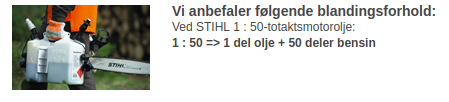
\includegraphics[]{stihl}
\end{figure}
Si at vi skal fylle på 2,5\enh{l} bensin på motorsagen vår, hvor mye olje må vi da tilsette?

\vsk \vspace{12pt}
\begin{comment}
Oppgave om hvilket dyr som er sterkest i forhold til vekten. Skaraben er verdens sterkeste.
\end{comment}

\op{lodd}
Du skal lage et lotteri der forholdet mellom antall vinnerlodd og taperlodd er $ \frac{1}{8} $. Hvor mange taperlodd må du lage hvis du skal ha 160 vinnerlodd?

\eksop{2PV23D1}{2pv23d1opg2}
På et kart er avstanden mellom to byer 40 cm. I virkeligheten er avstanden 20 km.
Bestem målestokken til kartet.

\eksop{2PV24D1}{2pv24d1opg3}
300 meter i virkeligheten tilsvarer 2\,cm på et kart. Bestem målestokken til dette kartet.

\eksop{2PH24D1}{2ph24d1opg1}
På et kart er avstanden mellom to byer 10 cm. I virkeligheten er denne
avstanden 5 km.
Bestem målestokken til kartet.

\op{forh}
De fleste brus inneholder ca 10\enh{g} karbohydrater per 100\enh{g}. En type saftsirup inneholder 44\enh{g} karbohydrater per 100\enh{g}. Saften skal lages med 2 deler sirup og 9 deler vann. \os

Hvor mange karbohydrater per 100\enh{g} inneholder ferdig utblandet saft? \os

\mers{I denne oppgaven går vi ut ifra at både 1\,dl vann og 1\,dl saftsirup veier 100\,g.}
\newpage

\grubeksoprecc{gv25d1opg2}{GV25D1}
Sander spilte håndballcup. Etter to kamper hadde han skåret på 11 av 20 skudd.
\abc{
\item Hvor mange prosent av skuddene scoret han på?
}
Skåringsprosenten økte til 60\,\% etter ti nye skudd i den tredje kampen.
\abcs{2}{
\item Hvor mange av de ti siste skuddene skåret Sander på?
}

\grubop{1ph23d1opg2} (1PH23D1)
\st{
\textbf{Ni av ti nordmenn bruker sosiale medier} \\
88\% av nordmenn bruker sosiale medier.
De siste fem årene har antall nordmenn som bruker sosiale
medier, økt med 8 prosentpoeng.
}
Opplysningene ovenfor er hentet fra ssb.no.\os
\abc{
\item Vil du si at overskriften samsvarer med første setning i teksten?
Begrunn svaret ditt.
\item Hvor mange prosent tilsvarer økningen på 8 prosentpoeng?
}

\grubop{opgbrokvisproendrb}
Bruk \rref{vekstfaktfrm} og \rref{proendra} til å utlede formelen i \rref{proendrb}. 

\grubeksoprecc{gv26d1opg9}{GV26}
Et bilde som skissert under skal forstørres slik at rektangelet blir 60\,cm langt og 40\,cm bredt. Hva blir sidelengden til trekanten\\ etter forstørringen? (Sidelengden som var 7\,cm.)
\fig{gv26d1opg9}


\grubeksoprecc{1ph21d2opg5}{1PH21}
Angelica har laget blåbærsaft. Saften inneholder 10\,\% sukker. \\ Angelica synes saften
er sur og vil lage en ny saftblanding med 50\,\% mer sukker. \os

Hvor mange prosent sukker vil den nye saftblandingen inneholde?

\grubeksoprecc{1pv25d1opg2}{1PV25D1}
I en kommune fikk Arbeiderpartiet 40\% av stemmene ved forrige valg. Senterpartiet
fikk 20\% av stemmene. En meningsmåling viser at begge partiene har økt sin
oppslutning med 5 prosentpoeng siden valget. \os

Hvilket parti har hatt størst prosentvis framgang? Grunngi svaret.

\grubeksoprecc{1ph25d2opg5}{1PH25D2}
Verdien av en aksje har gått ned med 23\%.
Hvor mange prosent må verdien øke med for at aksjen skal ha samme verdi som før
nedgangen?

\grubeksoprecc{1pv26d1opg6}{1PV26D1}
Prisen for en vare settes opp med 10\%.
Litt senere settes prisen ned igjen med 10\%. \os

Koster varen nå mer enn, mindre enn eller det samme som den gjorde før de to
prisendringene? Grunngi svaret ditt.

\grubeksoprecc{1pV26d1opg7}{1PV26D1}
Christoffer har kjøpt ny båt. Båtens verdi er 850 000 kroner. Anta at verdien vil falle
med 20\% det første året og så med 6\% per år de neste fem årene. \os

Sett opp et uttrykk som kan brukes for å regne ut båtens verdi etter seks år.

\grubop{opgbrokpofolgende}
Bruk uttrykket $(1+x)(1-x)$ som utgangspunkt for å avgjøre om følgende påstander er riktige:
\begin{center}
	\small
	\begin{tabular}{p{2cm}|p{8cm}}
		\hline
		Påstand 1 & En økning og en påfølgende reduksjon av en verdi vil gi en lavere verdi enn utgangspunktet. \\ \hline
		Påstand 2 & En økning og en påfølgende reduksjon av en verdi vil gi en høyere verdi enn utgangspunktet. \\ \hline
		Påstand 3 & En økning og en påfølgende reduksjon av en verdi gi lik verdi som utgangspunktet. \\ \hline
		Påstand 4 & En reduksjon og en påfølgende økning av en verdi vil gi en lavere verdi enn utgangspunktet. \\ \hline
		Påstand 5 & En reduksjon og en påfølgende økning av en verdi vil gi en høyere verdi enn utgangspunktet. \\ \hline
		Påstand 6 & En reduksjon og en påfølgende økning av en verdi gi lik verdi som utgangspunktet. \\ \hline
	\end{tabular}
\end{center}

\grubeksoprecc{2pv23d2opg6}{2PV23D2}
Bredden til et rektangel skal minskes med en gitt prosentandel, og lengden skal økes med den
samme prosentandelen. \os

Avgjør hvilken av de tre påstandene nedenfor som er riktig. Grunngi svaret ditt.
\begin{enumerate}
	\item Arealet til rektangelet vil bli mindre.
	\item Arealet til rektangelet vil bli større.
	\item Om arealet til rektangelet blir større eller mindre kommer
	an på hvilken prosentandel vi bruker.
\end{enumerate}

\grubeksoprecc{2pv24d1opg5}{2PV24D1}
Nora skal kjøpe bagetter med følgende tilbud: ''2 for 32 kroner eller
4 for 48 kroner''. Hvor mange prosent lavere blir prisen per bagett dersom hun kjøper fire
i stedet for to?

\end{document}

